\chapter{Analyse}

Ziel dieser Arbeit ist es ein Modell zu entwickeln, dass es ermöglicht große Mengen von Bildern zu gruppieren. Durch die großen Mengen an Daten die zu verarbeiten sind, sollen \textit{state of the art} Verfahren genutzt werden, die speziell hierauf ausgelegt sind. Der erste der Teil der Analyse befasst sich daher mit dem Bereich des \textit{Machine Learning}. Hier handelt es sich um keine umfängliche Einführung. Es werden Methoden beleuchtet, die zur Komprimierung und Gruppierung von Daten dienen und die Basis des hier vorgeschlagenen Modells bilden. Anhand der Anforderungen und Annahmen wird dann ein unüberwachtes Lernverfahren ausgewählt, dass zu Gruppierung von Bildern dient und in den folgenden Kapiteln weiter ausgearbeitet und realisiert wird. \newline
Im zweiten Teil sollen Möglichkeiten untersucht werden, aus Bildern Features zu gewinnen, welche als Eingabe für das Modell dienen. Um einen Überblick über Features in der Bildverarbeitung zu gewinnen, sollen zunächst einige Feature-Detektoren bzw. Deskriptoren für unterschiedlicher Anwendungsfälle aufgeführt werden. Heute ist es kaum vorstellbar, dass ein Feature-Deskriptor jeden möglichen Anwendungsfall abdecken kann. Daher soll abschließend der Fokus dieser Arbeit festgelegt werden: Sollen beispielsweise Gesichter oder Szenen erkannt werden? Sollen Objekte erkannt werden und wenn ja, beliebige Kategorien? Anhand der gewonnen Erkenntnisse wird dann entschieden, welche Eigenschaften der hier verwendete Feature-Deskriptor aufweisen soll. 

%Ein Gruppieren von Bildern anhand ihrer Deskriptoren ist ohne weitere %Verarbeitung kaum möglich. Zum einen besitzen die Feature-Deskriptoren viele %Komponenten, zum anderen liegen pro Bild selbst viele Deskriptoren vor (bei %gängigen Größen ca. 20 - 3000 Deskriptoren).\newline

\section{Verwendung der GPU}

Zum Aufbauen eines Modells werden mehrere Zehn- bis Hunderttausend Features verarbeitet werden. Viele der Verfahren, die der Erzeugung solcher Modellen zu Grunde liegen, wurden in den vergangenen Jahren durch die Verwendung der GPU statt der CPU beschleunigt. Bei der Betrachtung geeigneter Ansätze wird daher auch berücksichtigt, ob und wie eine Beschleunigung durch parallele Verarbeitung erzielt werden kann. Gerade bei großen Datenmengen und einer enormen Datenparallelität können Probleme durch GPUs um ein vielfaches schneller gelöst werden als durch CPUs. Da Nvidias CUDA an der Hochschule Hannover sowohl gelehrt als auch zu Forschungszwecken genutzt wird und sich CUDA auch international in Forschung und Wirtschaft etabliert hat, soll die Plattform als technische Basis dienen. 

\section{Machine Learning}

\textit{Machine Learning}ist ein Teilgebiet der künstlichen Intelligenz und wird genutzt um System zu entwerfen, die nicht explizit programmiert werden. Stattdessen Lernen diese Systeme: Lernen bedeutet in diesem Kontext, dass eine System durch eine Eingabe seine Struktur verändert, um so die erwartete Leistung zu steigern. Dabei ist \textit{Machine Learning} ein interdisziplinäres Feld: Es sind sowohl Computerwissenschaften, Statistik als auch biologische und kognitive Wissenschaften involviert. Bisher haben sich viele Anwendungsfälle für \textit{Machine Learning} Verfahren ergeben, die bis in den Alltag reichen. Einige Beispiele sind:

\begin{itemize}
	\item \textbf{Optical Character Recognition (OCR)} Unter OCR wird das Übersetzen eines (hand-)geschriebenen Textes in eine digitales Dokument bezeichnet. Beispielsweise kann so das Einfügen von Daten in CRM / ERP System automatisiert werden.
	\item \textbf{Spam Filterung} Das automatische Erkennen von unerwünschten E-Mails, die Werbung enthalten oder Betrugsversuche sind, ist inzwischen bei jedem Mail-Anbieter Teil des Angebots.
	\item \textbf{Spracherkennung} Auch eine Spracherkennung ist bereits auf den meisten digitalen Assistenten verfügbar und wird sogar zur Steuerung der häuslichen Elektronik verwendet.
	\item \textbf{Anomalie Erkennung} Digitale Geldtransaktionen werden heute von Algorithmen überwacht, die Abweichungen im Zahlungsverhalten beobachten. Wird eine ungewöhnlich hohe Summe überwiesen oder abgehoben, kann so informiert und auch interveniert werden.
\end{itemize}

All diese Verfahren nutzen eine große Menge an Trainingsdaten, um so ein Modell zu generieren, welches eine Klassifizierung weiterer Daten ermöglicht. Beispielsweise müssen bei einem System zur Spam-Filterung sowohl \enquote{normale} als auch Spam E-Mails verwendet werden, eine Spracherkennung benötigt digitale Aufnahmen von Wörtern und Sätzen zum Lernen, etc.
Nach dem Aufbau des Modells findet dann durch das System die Klassifizierung von Test- bzw. realen Daten statt. Es wird beispielsweise bei OCR entschieden, welches digitale Pendant zum vorliegenden Zeichen gehört oder bei der Spam-Filterung wie hoch die Wahrscheinlichkeit ist, dass es sich bei einer Mail um Spam handelt. Diese Trainings- und Testphase sind typisch für \textit{Machine Learning} Ansätze. Allgemein eignet sich dieser Ansatz:

\begin{itemize}
	\item Um Beziehungen und Muster in den Daten zu entdecken, die nicht offensichtlich sind. Genau mit dieser Fragestellung beschäftigt sich die Disziplin des \textit{Data Mining}. Hierfür werden u.a. maschinelle Lernalgorithmen genutzt.
	\item Wenn kein klassischer Algorithmus für die Problemstellung entworfen werden kann oder das Programm zu komplex ist, als das es von Menschen kodiert und gewartet werden könnte.
	\item Um neue Informationen einzubeziehen. Das Modell basiert auf den Daten, daher kann das System sich theoretisch durch neue Daten verändern und so der Situation anpassen.
\end{itemize}

\subsection{Lernverfahren}

Je nach Fragestellung haben sich unterschiedliche Methodiken entwickelt, um den Lernprozess in einem System abzubilden. Im Wesentlichen werden drei Arten des maschinellen Lernens unterschieden:

\begin{itemize}
	\item \textbf{Überwachtes Lernen (supervised learning)} Ein überwachtes Lernverfahren soll eine Funktion $f$ lernen, die Eingaben ($x$) ihren Ausgaben ($y$) zuordnet, sodass gilt: $y = f(x)$ . Diese Funktion wird anhand von Trainingsdaten gelernt, die demzufolge aus Paaren von Eingaben und ihren dazugehörigen Ausgaben bestehen.
	\item \textbf{Unüberwachtes Lernen (unsupervised learning)} Ziel unüberwachter Lernalgorithmen ist es, großen Mengen von nicht kategorisierten Daten zu gruppieren oder zu komprimieren. Dadurch können Beziehungen in den Daten entdeckt bzw. kompaktere Darstellungen erreicht werden.
	\item \textbf{Verstärkendes Lernen (reinforcement learning)} Beim verstärkenden Lernen hat ein Agent die Aufgabe ein vorgegebenes Ziel zu erreichen, indem er mit seiner Umwelt agiert. Die Umwelt ist dabei eine Menge von Zuständen zwischen denen der Agent durch eine Aktion wechselt. Dabei hat jede Aktion eine Belohnungen oder Bestrafungen zufolge. Der Agent optimiert dann sein Verhalten, um die erhaltenen Belohnungen zu maximieren.
\end{itemize}

Beim überwachten Lernen ist es notwendig, dass sowohl Ursachen (Eingaben) als auch Effekte (Ausgaben) gemessen wurden. Hier sollen dann durch ein trainiertes Modell eine Vorhersage der Ausgabe abhängig von der Eingabe erfolgen. Beim unüberwachten Lernen hingegen sind die Eingaben latente Variablen. Das heißt sie sind nicht direkt gemessen worden, sondern durch mathematische Verfahren von Observationen abgeleitet. Dadurch ist ein exploratives Vorgehen möglich. Es können Beziehungen in den Daten entdeckt und Gruppierungen bzw. Klassifizierungen durchgeführt werden.

\subsection{Unüberwachte Lernverfahren im Kontext dieser Arbeit}

Für die Gruppierung des Bildmaterials eignen sich maschinelle Lernverfahren besonders, da sie zum einen auf eine große Menge an Trainingsdaten angewiesen sind, um ein nützliches Modell zu generieren und zum anderen eine parallele Verarbeitung begünstigen. In dieser Arbeit werden hierfür unüberwachte Lernverfahren aus folgenden Gründen genutzt:

\begin{itemize}
	\item Das Gruppieren bzw. Kategorisieren von Daten (\textit{Clustering}) ist selbst ein Teilgebiet innerhalb der unüberwachten Lernverfahren.
	\item Die Feature-Vektoren umfassen oft viele Komponenten, welche zur Kodierung der Eigenschaften erforderlich sind. Im Bereich des \textit{Machine Learning} gibt es Verfahren, welche die Feature-Vektoren auf ihre wesentlichen Komponenten analysieren und so eine kompaktere Darstellung erzeugen.
	\item Es sollen Darstellungen bzw. Strukturen in den Daten entdeckt werden, die nicht a priori bekannt sind. Ein überwachter Ansatz erfordert zum Training \textit{gelabelte} Daten, um Vorhersagen zu treffen. Da die gesuchten Strukturen aber gerade nicht bekannt sind, scheidet ein überwachter Ansatz aus.
\end{itemize}

Hieraus geht hervor, dass zum Gruppieren der Bild-Features ein \textit{Clustering} Verfahren notwendig ist. Diese Art von Algorithmen und einige ihrer Vertreter werden daher im Folgenden vorgestellt. Außerdem scheint es sinnvoll die Features vor dem Clustering aufzubereiten: Durch eine kompaktere Darstellung der Feature-Vektoren kann der notwendige Speicher reduziert und die Berechnung beschleunigt werden. Nach dem Clustering folgt daher einer Übersicht über den Bereich \textit{Dimensionality Reduction (Reduzierung der Dimensionalität}: Diese Art von Algorithmen hat die Kompression von Daten zum Ziel.

\textbf{Clustering-Verfahren} quantisieren die Daten in Gruppen. Eine Gruppe steht hier für ein semantisches Merkmal und vertritt eine Menge von konkreten Daten. Unter Clustering Verfahren fallen Algorithmen wie k-means, hierarchical clustering oder etwa das Gaussian Mixture Model.\newline
Ein Clustering Algorithmus hat in dem Kontext dieser Arbeit das Ziel, eine großen Menge Feature-Deskriptoren auf die Wesentlichen zu reduzieren. Durch diese Quantisierung in $n$ Gruppen müssen, bei einer Bewertung eines neuen Deskriptors, nur Vergleiche mit $n$ Deskriptoren durchgeführt werden, statt mit jedem Deskriptor der Ursprungsmenge.\newline

\textbf{Verfahren zu Reduzierung der Dimensionalität} nehmen an, dass es eine unterliegende Struktur gibt, welche entdeckt werden kann. In diesem Fall vertreten die Dimensionen semantische Merkmale. Methoden wie beispielsweise die Hauptkomponentenanalyse bilden die Feature-Vektoren auf einen Raum niederer Dimensionen ab. \newline
Ein moderneren Ansatz für diesen Zweck ist die Verwendung neuronaler Netze. Ein Autoencoder ist ein spezielles neuronales Netzwerk, welches für das Lernen einer komprimierten Darstellung von Daten verwendet wird. Das Konzept des Autoencoders reicht zwar bis in 80er Jahre zurück, eine Methode zum Training tiefer Netze ist aber erst 2006 von Hinton entwickelt worden.\newline

Um einen kompakteren Feature-Deskriptor zu erzeugen soll ein Autoencoder verwendet werden. Ein Mehrstufiger Autoencoder kann mit jeder Schicht einen kompakteren Deskriptor erzeugen und kodiert die gelernten Informationen in den Gewichten. Der Autoencoder bringt darüber hinaus den Vorteil mit sich, das seine Architektur bereits auf eine parallele Verarbeitung ausgelegt ist und nicht \enquote{extra}berücksichtigt werden muss. Des Weiteren sind klassische Methoden wie die Hauptkomponentenanaylse bereits zahlreich betrachtet worden. Ein Autoencoder hingegen ist in diesem Bereich, im Vergleich, ein neuer Vertreter, dessen vielfältige Einsatzmöglichkeiten immer noch erforscht werden. \todo{Vorteile Autoencoder}. \newline  
Um die Features zu Gruppieren soll ein k-means Clustering Verfahren verwendet werden. Anhand der durch k-means gewonnen Cluster kann eine Histogrammdarstellung für Features erzeugt werden. Die Kombination diese Verfahren wird Bag of Visual Words genannt und lehnt sich an das Bag of Words Modell an. Hinsichtlich der Berechnung durch eine GPU, sind diese Verfahren auch gut geeignet: Die Familie der k-means Algorithmen enthält viele Algorithmen die lange etabliert sind und bereits für die parallele Ausführung auf Grafikkarten adaptiert wurden. Das parallele Verarbeiten von Histogrammen ist ein Lehrbuchbeispiel für den Einsatz von Grafikkarten, da es durch parallelen Reduzierung, ein Muster für einige Probleme, erreicht werden kann.

\section{Autoencoder}

Durch den Aufschwung des maschinellen Lernens in den letzten Jahren sind neuronale Netze stark in den Fokus der Industrie und Wissenschaft gerückt. Solche künstlichen neuronalen Netze werden genutzt, um aus Beispielen Muster zu lernen und diesen Wissen zu transferieren. 
Ein spezielles neuronales Netzwerk zum unbeaufsichtigten Lernen ist der Autoencoder. Diese Art von Netzwerk lernt selbstständig eine komprimierte Darstellung der Eingabe. 
Als erstes wird im folgenden Abschnitt der Aufbau und die Funktionsweise eines Autoencoders erläutert. Darauf aufbauend werden zwei Erweiterungen des Autoencoders vorgestellt: Der Stacked Autoencoder und der Denoising Autoencoder. Ersterer wird verwendet, um effektiv tiefe Netzwerke zu konstruieren, letzterer ermöglicht eine korrekte Konstruktion aus verzerrten Daten.

\subsection{Aufbau und Funktionsweise}

Ein Autoencoder (AE) ist ein spezielles neuronales Netzwerk, dass eine komprimierte Kodierung der Eingabe lernt. Ein Autoencoder versucht die Daten zu rekonstruieren und kann daher unbeaufsichtigt lernen: Die rekonstruierten Daten können anhand einer Distanzmetrik mit den Originaldaten verglichen werden. Anschließend kann die Größe des Fehlers berechnet werden und durch \textit{Backpropagation} die Gewichtesmatrix aktualisiert werden \cite{ssn1997}.
Um die Originaldaten als Ergebnis erhalten zu können, muss die Anzahl der Neuronen des \textit{Input Layers} der Anzahl der Neuronen im \textit{Output Layer} entsprechen. Die Anzahl der Neuronen im \textit{Hidden Layer} ist geringer, um die komprimierte Darstellung des Features zu erreichen. Werden mehrere \textit{Hidden Layer} verwendet, so nimmt die Neuronenanzahl von Schicht zu Schicht ab um die Anzahl der Komponenten weiter zu verringern. Dieser Vorgang ist die Enkodierung und liefert die gewünschte komprimierte Abbildung. Die Dekodierung ist umgekehrt aufgebaut, um das Original aus der komprimierten Repräsentation Schicht für Schicht zu rekonstruieren. Wie gut die Dekodierung gelungen ist, lässt sich dann anhand eines Vergleichs der Distanz des Original und der Rekonstruktion bewerten.\newline
Formal wird ein Eingabevektor $x \in [0,1]^n$ auf einen Vektor $y \in [0,1]^p$, mit $p < n$, abgebildet: 
$$y = encode_{W,b}(x) = s(Wx + b)$$
$W$ ist die Gewichtsmatrix der Größe $n \times p$ und $b$ der Bias-Vektor. Diese Parameter werden durch den Autoencoder optimiert. Die Darstellung $y$ wird in diesm Kontext auch als \textit{code} bzw. latente Variablen bezeichnet. Die Rekonstruktion erfolgt durch die Dekodierungsfunktion. Der Vektor $z \in [0, 1]^n$ berechnet sich durch: 
$$z = decode_{W', b'}(y) = s(W'y + b')$$
In Abbildung \ref{img:example_ae} ist ein Autoencoder abgebildet der als Eingabe einen Vektor $x \in [0,1]^4$ entgegen nimmt. Dieser wird auf den Vektor $y$ mit drei Komponenten abbildet, da der \textit{Hidden Layer} drei Neuronen enthält. Die Rekonstruktion $z$ aus $y$ erfolgt dann durch die Berechnung der Dekodierungsfunktion.

\begin{figure}
	\centering

	\begin{tikzpicture}[shorten >=1pt,->,draw=black!50, node distance=\layersep]
    \tikzstyle{every pin edge}=[<-,shorten <=1pt]
    \tikzstyle{neuron}=[circle,fill=black!25,minimum size=17pt,inner sep=0pt]
    \tikzstyle{input neuron}=[neuron, fill=green!50];
    \tikzstyle{output neuron}=[neuron, fill=red!50];
    \tikzstyle{hidden neuron}=[neuron, fill=blue!50];
    \tikzstyle{annot} = [text width=6em, text centered]

    % Draw the input layer nodes
    \foreach \name / \y in {1,...,4}
        \node[input neuron, pin=left:$x_{\y}$] (I-\name) at (0,-\y) {};

    % Draw the hidden layer nodes
    \foreach \name / \y in {1,2,3}
        \path[yshift=-0.5cm]
            node[hidden neuron] (H-\name) at (\layersep,-\y cm) {$y_{\y}$};
    
    % Draw the output layer nodes
    \foreach \name / \y in {1,...,4}
        \node[output neuron,pin={[pin edge={->}]right:$z_{\y}$}, right of=H-3] (O-\name) at (\layersep,-\y) {};

    % Connect every node in the input layer with every node in the
    % hidden layer.
    \foreach \source in {1,...,4}
        \foreach \dest in {1,2,3}
            \path (I-\source) edge (H-\dest);

    % Connect every node in the hidden layer with the output layer
    \foreach \source in {1,2,3}
        \foreach \dest in {1,...,4}
        	\path (H-\source) edge (O-\dest);

    % Annotate the layers
    \node[annot,above of=H-1, node distance=1.5cm] (hl) {Hidden Layer};
    \node[annot,left of=hl] {Input Layer};
    \node[annot,right of=hl] {Output Layer};
	\end{tikzpicture}

	\caption{Beispiel eines simplen Autoencoders}
	\label{img:example_ae}
\end{figure}

\subsection{Stacked Denoising Autoencoder}

Von Hinton and Salakhutdinov wurde 2006 das Konzept des Stacked Autoencoders eingeführt, um einige Probleme mit herkömmlichen Autoencoder zu überwinden \cite{dae2006}. Bei Netzwerken mit mehr als einem \textit{Hidden Layer} erzielt die Gradientenabstiegs-Methode, aufgrund der zunehmenden Verzerrung der Gradienten, bei der Rückpropagierung keine guten Ergebnisse mehr. In vielen Ansätzen wurde auch eine zufällige Initialisierung der Gewichte gewählt. Hier besteht die Gefahr, dass der Algorithmus in einem lokalen Optimum verbleibt. Wenn die anfänglichen Gewichte hingegen bereits nah an einer guten Lösung liegen, sinkt die Wahrscheinlichkeit eines lokalen Optimums. Aus diesem Grund wurde das Pretraining für Autoencoder mit mehr als einer Schicht vorgeschlagen. In diesem Training wird jedes Paar aneinanderliegender Schichten als ein Autoencoder aufgefasst und einzeln trainiert. Das Pretraining besteht aus drei Schritten, die wiederholt werden, bis alle Autoencoder trainiert sind.

\begin{enumerate}
	\item Es wird der aktuelle Autoencoder trainiert. Zu Beginn besteht dieser aus dem \textit{Input} und folgendem \textit{Hidden Layer}.
	\item Nun wird der Decoder des trainierten Autoencoders entfernt und ein neuer Autoencoder erzeugt. Dieser besitzt den \textit{Hidden Layer} des trainierten Autoencoders als \textit{Input Layer}.
	\item Das Training wird mit dem neuen Autoencoder fortgeführt.
\end{enumerate}

Ein Denoising Autoencoder \cite{sda2010} dient dazu, eine korrumpierte Eingabe zu korrigieren. Die Korruption ist hier als Rauschen bzw. Verzerrung (\textit{noise}) aufzufassen. In vielen Arten von Features, z.B. Bildern oder Audiomaterial, sind Verzerrungen bereits in den Daten vorhanden, beeinflussen die Semantik des Ganzen aber kaum. Daher soll der Autoencoder dies bereits berücksichtigen, indem er nicht direkt mir der Eingabe $x$ arbeitet. Stattdessen wird $x$ auf die korrumpierte Eingabe $\widetilde{x}$ durch ein stochastisches Verfahren abgebildet. In der Enkodierungsfunktion wird dann $\widetilde{x}$ statt $x$ verwendet: 
$$encode_{W,b}(\widetilde{x}) = s(W\widetilde{x} + b)$$
In der Praxis hat sich zur Korruption der Eingabe die \textit{masking corruption} Technik bewährt: Hierbei werden 20\% bis 50\% der Neuronen des \textit{Input Layers} zufällige ausgewählt und werden \enquote{genullt}. Auf diese Weise wird vermieden, dass der Autoencoder nur von bestimmten Teilmengen an Neuronen abhängt  \cite{pda2012}.

\subsection{Hyperparameter}

Bisher wurde das Netzwerk und die Parameter die es optimiert, die Gewichte $w$ und der Bias-Vektor $b$, betrachtet. Darüber hinaus gibt es eine Reihe von Parametern, die Hyperparameter, die vor Anwendung des Modells festgelegt werden müssen. Die wesentlichen Hyperparameter für neuronale Netze sollen hier vorgestellt und ihr Einfluss auf das Modell erläutert werden. Die aufgeführten Standardwerte wurden bei einer Vielzahl von Modellen beobachtet, gelten aber nicht uneingeschränkt für jeden Anwendungsfall \cite{pda2012}. 
%https://arxiv.org/pdf/1206.5533.pdf

\begin{itemize}
	\item \textbf{Initiale Lernrate} Bei gradientenbasierten Vefahren wird in jeder Iteration der Fehler zurückpropagiert. Dies wird in den meisten Fällen zu einer zu schnellen Anpassung des Netzes führen und es \enquote{vergisst} schnell, was es bereits gelernt hat. Aus diesem Grund werden die berechneten Fehler mit der Lernrate (\textit{learning rate}), einem kleinen Wert, multipliziert. Praktisch wird für die Lernrate ein Wert kleiner 1 und größer $10^{-6}$ verwendet.
	\item \textbf{Anzahl der Trainingsiteration} Eine Iteration entspricht einem \textit{forward} und \textit{backward pass} einer kleinen Teilmenge (ein \textit{batch}) der gesamten Trainingsmenge. Eine zu große Anzahl an Iterationen führt zu einer Überanpassung des Netzes an die Trainingsdaten, daher sollte gestoppt werden, wenn sich andere Metriken nicht mehr verbessern.
	\item \textbf{Anzahl der Exemplare pro Trainingsiteration} (\textit{batch size)} Je größer die \textit{batch size}, desto mehr Trainingsexemplare werden pro Iteration verarbeitet. Durch einen größeren Wert kann die Berechnung beschleunigt werden, allerdings ist auch mehr Speicher erforderlich. In der Praxis liegt der Wert für diesen Parameter meist zwischen 16 und 128 (Zweierpotenzen). 
\end{itemize}

\subsection{Autoencoder für Bild Features}
\label{AEFeatures}

Ein populäres Beispiel für die Verwendung von Autoencodern ist das Klassifizieren von Ziffern in einem Bild. Solch ein Netzwerk arbeitet direkt mit den Pixeln des Bildes: Bei einem Bild mit $m \times n$ Pixeln, umfasst die erste Schicht ebenfalls $m \times n$ Neuronen, für jeden Pixel Eines. Wie üblich umfassen die folgenden Schichten weniger Neuronen. Durch eine abschließende Schicht zur Klassifizierung wird das Bild schließlich eingeordnet. Hier soll aber nicht direkt mit den Pixeln des Bildes gearbeitet werden, sondern mit Feature-Vektoren. Für die Extraktion geeigneter \textit{keypoints} hat sich der SIFT-Detektor bewährt, der Deskriptor hat jedoch bereits eine zu kompakte Darstellung um ein tiefes Netzwerk aufzubauen. Es muss daher ein Deskriptor ausgewählt oder konstruiert werden, der initial viele Komponenten umfasst, die durch den Autoencoder reduziert werden. Auf diese Weise ist auch die Entwicklung weiterer Deskriptoren denkbar, die explizit keine Rücksicht auf eine kompakte Darstellung nehmen, sondern möglichst viele Informationen kodieren. Anschließend kann nach Konstruktion eines entsprechenden Autoencoders getestet werden, inwieweit sich der Deskriptor komprimieren lässt.

\section{Bag of Visual Words}

Das Bag of Visual Words lehnt sich an das Bag of Words Modell aus dem Bereich Information Retrival an. Daher soll zunächst die Funktionsweise des Bag of Word Modells erläutert werden, um darauf aufbauend den Bag of Visual Words einzuführen.\newline 
Der Bag of Words wird zur Klassifizierung von Dokumenten genutzt. Beim Bag of Words wird das Auftreten jedes Wortes in einem Dokument gezählt und durch die Anzahl aller Wörter im Vokabular dividiert, um so einen normalisierten Wert zu erhalten, welcher die relative Häufigkeit eines Wortes angibt. Das Vokabular wird \textit{Codebook} genannt, die Wörter werden auch als \textit{Codewords} bezeichnet.\newline
Dieses Modell wurde von der digitalen Bildverarbeitung adaptiert \cite{bok2004}. Es wird anhand der Features von Trainingsbildern ein visuelles Vokabular gelernt, das zur Klassifizierung von Bildern dient. Die Features können aber nicht direkt statt der Worthäufigkeit verwendet werden: Ein Wort ist ein diskreter Wert der direkt verglichen werden kann, ein Feature hingegen ist ein Vektor in einem hochdimensionalen Raum, der Eigenschaften beschreibt. Um konkrete Werte zu erhalten, ist es notwendig, die Vektoren zu quantisieren. Die quantisierten Vektoren entsprechen dann den \textit{Codewords} und werden in diesem Kontext auch \textit{Visual Words} genannt. \newline
Zunächst wird die Funktionsweise des Bag of Visual Words im folgenden Abschnitt näher betrachtet. Dem schließt eine Betrachtung des Kernstücks des Algorithms an: Das Clustering der Features. Hier wird ein k-means Algorithmus, Llyods heuristische Variante, verwendet. Es wird eine gängige sequentielle Implementierung angeführt, auf deren Basis dann die Parallelisierbarkeit durch Grafikkarten untersucht wird.\newline
Bei der Einordnung eines Bildes wird ein Histogramm der Visual Words generiert, daher wird im Anschluss ein sequentieller Histogramm Algorithmus vorgestellt, der auf Parallelisierbarkeit geprüft wird.

\subsection{Funktionsweise}

Der Bag of Visual Words besteht aus einer Trainings- und Testphase, wie in Abbildung \ref{img:bovw} dargestellt. Die Extraktion der Features ist beiden Phasen vorgelagert.\newline
Zu Beginn erfolgt die Trainingsphase, das Clustering der extrahierten Features. Das so erzeugte \textit{Codebook} ist das Modell, gegen das anschließend getestet werden kann. Die Idee ist, dass ähnliche Feature-Vektoren nah beieinander im Raum liegen und somit in die gleiche semantische Kategorie gehören. Durch einen Clustering Algorithmus wie k-means kann die Größe des \textit{Codebooks} bestimmt werden. Wird für $k$ ein große Zahl gewählt, wird ein Vokabular von Exemplaren aufgebaut, ein kleines $k$ hingegen erkennt eher Kategorien. Die Schwerpunkte der Cluster vertreten dann eine Menge von ähnlichen Features und bilden das \textit{Codebook} bzw. Modell.\newline
Der Testprozess erzeugt nun, auf Basis des \textit{Codebooks}, die \textit{Visual Words} von Bildern. Hierfür werden die Features eines Bildes extrahiert und ein Histogrammalgorithmus ermittelt die Verteilung der \text{Visual Words}: Für jedes Feature wird das ähnlichste \textit{Visual Word} des \textit{Codebooks} bestimmt und die entsprechende Klasse inkrementiert. Wird dieser Prozess auf zwei Bilder angewendet, so können die resultierenden Histogramme miteinander verglichen werden (z.B. mit dem \textit{MSE (mean squared error) als Metrik}.

\begin{figure}
	\centering
	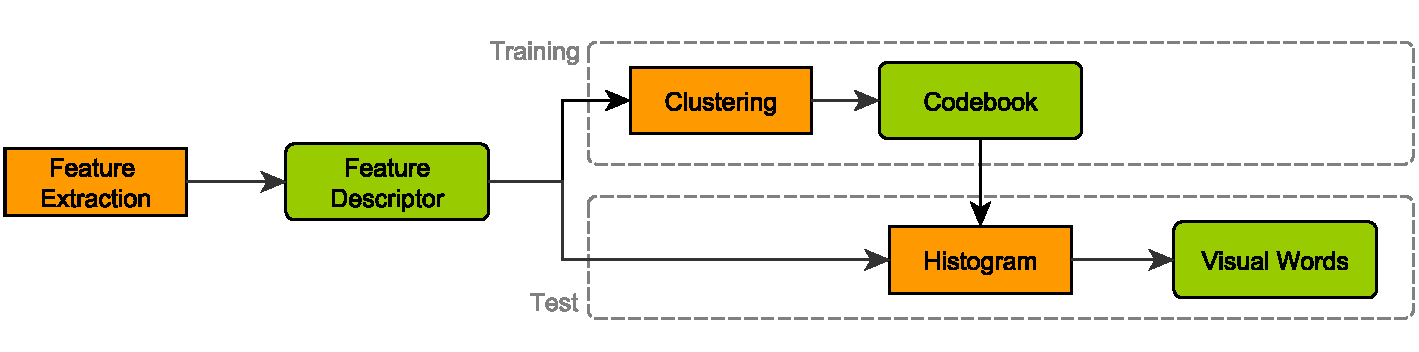
\includegraphics[scale=0.65]{images/bovw_process.pdf}
	\caption{Training- und Testprozess des Bag of Visual Word Modells.}
	\label{img:bovw}
\end{figure}

\subsection{Lloyds Algorithmus}

Im Grundlagenkapitel wurde bereits Lloyds Algorithmus eingeführt, hier soll zunächst näher auf die sequentielle Ausführung eingegangen werden, um anschließend eine mögliche Parallelisierung zu diskutieren. Im nachfolgenden Codelisting ist der Ablauf des Algorithmus in Pseudocode beschrieben. Als Parameter werden die Punkte $P$ und die Anzahl der zu bildenden Cluster $k$ erwartet. In Zeile 2 findet die Auswahl der initialen Schwerpunkte der Cluster statt. Die Zuordnung von Punkten zu Clustern erfolgt in Zeile 7: $argminD$ wählt den Cluster aus, dessen Varianz am Wenigsten bei Aufnahme des Punktes $p_{i}$ steigt. Abschließend wird die Aktualisierung der Schwerpunkte aller Cluster in der Schleife in Zeile 8 und 9 durchgeführt.

\lstset{language=C}
\begin{lstlisting}[mathescape=true]
kmeans_lloyd ($P, C, k$)
	initialisierung
	until convergence
		$C_{j} = 0, j = 1, ..., k$
		for each $p_{i} \in P$
			for each $c_{j} \in C$
				$c_{j} = argminD(c_{j}, p_{i})$		
		for each $c_{j} \in  C$
			$c_{j} = \frac{1}{|c_{j}|} \sum_{n_{i} \in c_{j}} n_{i}$
\end{lstlisting}

Die Initialisierungsphase muss für die Parallelisierung nicht beachtet werden: Sie nimmt nur wenig Zeit in Anspruch und wird einmalig zu Beginn ausgeführt. Die Anderen beiden Schritte des Algorithmus bergen mehr Potential: In Zeile 5 bis 7 wird die Varianz jedes Cluster-Vektor Paares berechnet. Da die Berechnung der Varianz eines Paares unabhängig von der eines anderen ist, kann die Berechnung aller Varianzen parallel erfolgen. Nachdem für einen Durchgang die Veränderung der Mitgliedschaft von Vektoren zu Clustern berechnet wurde, müssen die Cluster-Schwerpunkte aktualisiert werden. Auch die Berechnung der neuen Schwerpunkte der Cluster kann unabhängig voneinander erfolgen: Die Vektoren aus denen der Mittelwert berechnet wird, sind genau einem Cluster zugeordnet.

% http://www.know-center.tugraz.at/download\_extern/papers/latex8.pdf

\subsection{Histogramme}

Ein sequentielles Histogramm kann als Programm in einer Schleife über die Daten ausgedrückt werden: Für jedes Element wird der Index der Klasse des Histogramms berechnet und um eins inkrementiert. Zur Normalisierung des Histogramms ist es anschließend notwendig, jede Klasse des Histogramms durch die Gesamtanzahl der Werte zu dividieren. Da es sich bei der Anzahl der Klassen jedoch um eine kleine Zahl, im Vergleich zur Anzahl der Elemente in den Daten, handelt, ist dieser Aufwand vernachlässigbar.
Um das Histogramm der Visual Words eines Bildes zu erzeugen, muss für jedes extrahierte Feature das nächste Visual Word bestimmt werden. Dies entspricht im nachfolgenden Pseudocode der doppelten Schleife über die Features $F$ und Cluster $C$ in Zeile 2 und 3. Der Index des nächsten Clusters wird dann in Zeile 4 durch $argmin D$ berechnet und in der nächsten Zeile wird das Histogramm $H$ an der entsprechenden Stelle inkrementiert.

\begin{lstlisting}[mathescape=true]
histogram ($P, C, H$)
	for each $p_{i} \in P$
		for each $c_{j} \in C$
			$k = arminD(c_{j}, p_{i})$ 
		$H_{k} = H_{k} + 1$		
	for $1 .. |H|$
		$H_{i} = H_{i} / |H|$
\end{lstlisting}

\section{Feature Deskriptoren}
\label{extraction}

Für die weitere Verarbeitung der Features ist es erstrebenswert, dass ihre Darstellung möglichst kompakt ist. Deskriptoren werden als Vektoren von Zahlen kodiert, die abhängig vom Verfahren Informationen über einen Pixel und seine Nachbarschaft oder auch ein ganzes Bild enthalten. Je größer die Anzahl der Einträge eines Vektors, desto größer wird der Speicherbedarf und Rechenaufwand.
Die erste Stufe des vorgestellten Modells sieht daher die Komprimierung der Feature-Vektoren durch einen Autoencoder vor. Auf diese Weise kann ein initial recht umfangreicher Feature-Vektor aufgebaut werden: Jede Stufe des Autoencoders lernt dann eine kompaktere Darstellung des Feature-Vektors bis zu einer gewünschten Untergrenze.\newline
Da für die vorliegenden Bilddaten der HsH keine speziellen Annahmen getroffen werden können, ist nicht bekannt was für eine Art von Deskriptor gute Ergebnisse liefern kann. In der Literatur findet sich eine große Anzahl an Verfahren zur Detektion und Extraktion von Features für etliche Zwecke. Um einen Überblick zu geben, sollen einige Vertreter angeführt, um den Leser einzuführen.
\newline 

\textbf{Local Binary Patterns} Die Local Binary Patterns (LBP) haben sich im Bereich der Gesichtserkennung erfolgreich etabliert. Eine Region um einen \textit{keypoint} wird hier als ein acht stelliger Bitstring kodiert. Das Verfahren kodiert jeden Pixel einer $3 \times 3$ großen Nachbschaft, außer den Pixel im Fokus, als 0 oder 1, abhängig ob die Intensität größer oder kleiner einem Schwellwert ist.\newline 

\textbf{Spatial Envelope} Torralba und Olivia \cite{mts2001} haben mit dem  \textit{Spatial Envelope} ein Verfahren entwickelt um die z.B. die Natürlichkeit oder Offenheit einen Szene zu beurteilen. Eine hohe Natürlichkeit weist zum Beispiel auf das Bild einer Landschaft hin: Hier kommen in der Regel kaum gerade vertikale und horizontale Linien vor, im Gegensatz zu Bildern, die von Menschen angefertigt wurden.\newline

\todo{Noch einen}\newline

\textbf{SIFT} \todo{Einleitung} Der Deskriptor besitzt zwar keine affine Invarianz, in praktischen Anwendungen werden jedoch auch mit skalierten, rotierten und verschobenen Objekten gute Ergebnisse erzielt. Mikolajczyk und Schmid haben 2005 SIFT mit anderen Deskriptoren (u.a. shape context, komplexe Filter, gradient location and orientation histogram, moment invariants, ...) verglichen und kamen zu dem Ergebnis, dass SIFT sehr gut hinsichtlich Präzison abschneidet \cite{idp2005}. Die Konstruktion des Deskriptors ist allerdings sehr aufwendig und die Beschreibung erfordert einen Feature-Vektor mit 128 Komponenten.\newline

In dieser Arbeit soll im weiteren eine Basis für das Gruppieren von Bildern durch Features bilden, in dem ein Anwendungsfall umgesetzt wird. \todo{SIFT toll für Objekterkennung, Coole keypoints aber deskriptor schon zu kompakt für AE, SIFT kps nehmen und daraus eigenen Deskriptor aufbauen, Dann gehts weiter im Konzept mit zusammenflanschen}